\documentclass{../c-lecture}

\subtitle{Introduction}

\begin{document}

\begin{frame}
  \titlepage{}
\end{frame}
\begin{frame}
  \frametitle{Outline}
  \tableofcontents{}
\end{frame}

\section{Introduction}

\begin{frame}
  \frametitle{Who I am?}
  \centering
  \textbf{Parham Alvani}\\
  \textbf{Ph.D. Student in Computer Networks}\\
  \vfill
  \textit{parham [dot] alvani [at] gmail [dot] com}
\end{frame}
\begin{frame}
  \frametitle{Contact Me}
  \begin{itemize}
    \item No instant messaging
    \item \color{Orange} Email is Awesome
  \end{itemize}
\end{frame}

\section{What is this course?}

\begin{frame}
  \frametitle{This Course}
  \begin{itemize}
    \item Introduction to Computer \& Programming
    \item How to use computers to solve our problems
    \begin{itemize}
      \item The problems are computational problems
    \end{itemize}
  \end{itemize}
\end{frame}

\begin{frame}
  \frametitle{This Course (cont’d)}
  \begin{itemize}
    \item What we learn
    \begin{itemize}
      \item Overall overview of computer organization
      \item Problem solving steps
      \begin{itemize}
        \item Algorithm design
          \item A programming language: the {\color{Orange} C}
      \end{itemize}
    \end{itemize}
  \end{itemize}
\end{frame}

\begin{frame}
  \frametitle{This Course (cont’d)}
  \begin{itemize}
    \item What we don’t learn
    \begin{itemize}
      \item In depth computer hardware/software details
      \begin{itemize}
        \color{Aquamarine}
        \item Computer Architecture
        \item Operating System
      \end{itemize}
      \pause%
      \item Most advanced algorithms
      \begin{itemize}
        \color{Aquamarine}
        \item Data Structure
        \item Algorithms
      \end{itemize}
      \pause%
      \item System programming using C
      \begin{itemize}
        \color{Aquamarine}
        \item Operating System
      \end{itemize}
      \pause%
      \item Other programming languages: Java, PHP, etc.
      \begin{itemize}
        \color{Aquamarine}
        \item Advanced Programming
        \item Web Programming
      \end{itemize}
      \pause%
    \end{itemize}
  \end{itemize}
\end{frame}

\begin{frame}
  \frametitle{This Course (cont'd)}
  Steps to learn a new language (English, French, … C, Java, Python, …)

  \begin{enumerate}
    \item Present: what is the new language (course slide)
    \item Practice: how to use the new language in practice (the example)
    \item Produce: use the language to create a new things (Lab, HW)
  \end{enumerate}
\end{frame}

\begin{frame}
  \frametitle{This Course (cont'd)}
  Learning Programming Language

  \begin{itemize}
    \item is not a pure theoretical course (mathematics, …)
    \begin{itemize}
      \item Reading, reading, reading, ….
    \end{itemize}
    \item is a practical course needs the product step
    \begin{itemize}
      \item Class, Reading, programming, programming, programming,…
    \end{itemize}
  \end{itemize}
\end{frame}

\begin{frame}
  \frametitle{This Course (cont'd)}
  Course Materials
  \begin{itemize}
    \item Lecture notes (slides) are in (simple) English
  \end{itemize}
\end{frame}
\begin{frame}[allowframebreaks]
  \frametitle{Agenda}
  \begin{itemize}
    \item Introduction
    \item Algorithm Design
    \item Basic Concepts
    \item Calculations
    \item Interaction
    \item Decision
    \item Iteration
    \item Function
    \item Array
    \item Pointer
    \item Struct
    \item File
    \item Misc.
  \end{itemize}
\end{frame}
\begin{frame}
  \frametitle{Grading}
  Major Parts + 5\% Extra
  \begin{table}
    \begin{tabular}{cc}
      \toprule

      Midterm &
      25\% \\

      \midrule

      Final &
      25\% \\

      \midrule

      Lab &
      15\% \\

      \midrule

      Homework &
      30\% \\

      \midrule

      Project &
      10\% \\

      \bottomrule
    \end{tabular}
  \end{table}
\end{frame}

\begin{frame}
  \frametitle{Extra Classes}
  Lab + TA Classes

  \begin{itemize}
    \item Lab:\@ A practical class
    \item TA:\@ More details, Practical aspects, Solving HW
    \item Homework are not accepted after solutions
  \end{itemize}
\end{frame}

\section{Computer organization}

\begin{frame}
  \frametitle{Computers: The Computing Machines}
  Computer Classififcation:
  \begin{itemize}
    \item \textbf{Supercomputers}:\@
    Weather forecast, Large scale simulation, \ldots
    \item \textbf{Mainframe computers}:\@
    The servers in large companies: Google, \ldots
    \item \textbf{Midsize computers}:\@
    The servers in CE department
    \item \textbf{Micro computers (also called PC)}:\@
    Our laptop
    \item \textbf{Pocket PCs}:\@
    Our mobile phones
  \end{itemize}
\end{frame}

\begin{frame}
  \frametitle{Computers}
  \begin{itemize}
    \item Computers are programmable machines capable of performing calculations (computation)
    \item Changing program leads to different operation
    \item Special-purpose machines
    \begin{itemize}
      \item Calculators, game-playing machines, \ldots
    \end{itemize}
    \item General-purpose computers
    \begin{itemize}
      \item Personal computers, notebooks, \ldots
    \end{itemize}
  \end{itemize}
\end{frame}

\begin{frame}
  \frametitle{Data Units}
  \begin{itemize}
    \item Computers are digital machines
    \item Data processed or stored in computer is represented as two-state values
    \begin{itemize}
      \item either 1 or 0 --- BInary digiTs (BIT)
      \item 1 Byte = 8 bits
      \item 1 kilobyte (KB) = 1024 bytes
      \item 1 megabyte (MB) = 1024 kilobyte
      \item 1 gigabyte (GB) = 1024 megabyte
    \end{itemize}
  \end{itemize}
\end{frame}

\begin{frame}
  \frametitle{Data Representation/Coding}
  \begin{itemize}
    \item How to represent our data by 0--1?
    \item In other word, there are some 0 and 1 in the computer, what is the meaning?
    \item {\color{YellowOrange} Coding (Representation Standards)}
    \item Major (common) representations (coding)
    \begin{itemize}
      \item Integer numbers: 1, 1000, -123, 0, \ldots
      \item Floating point numbers: 1.1, 11.232, -12.23, \ldots
      \item Characters: ``A'', ``B'', ``@'', \ldots
    \end{itemize}
  \end{itemize}
\end{frame}

\begin{frame}
  \frametitle{Integer Number Coding}
  \begin{itemize}
    \item There are different representations
    \item One of the (simple) coding is sign-magnitude coding
    \begin{itemize}
      \item If we have $n$ bit for coding integer
      \item The left bit (the MSB): sign
      \item $n-1$ bits: magnitude
    \end{itemize}
  \end{itemize}
  \begin{table}
    \begin{tabular}{ccc}
      \toprule
      4 & 0000 & 0100 \\
      \midrule
      -4 & 1000 & 0100 \\
      \midrule
      0 & 0000 & 0000 \\
      \midrule
      -0 & 1000 & 0000 \\
      \bottomrule
    \end{tabular}
  \end{table}
\end{frame}

\begin{frame}
  \frametitle{Integer Number Coding}
  Two's Complement
\end{frame}

\begin{frame}
  \frametitle{Floating Point Number Coding (IEEE 754)}
  \begin{itemize}
    \item Usually, this coding pattern
    \item Two precisions:
    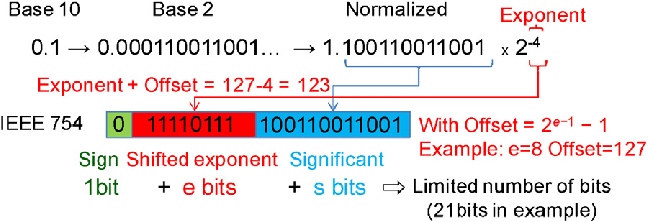
\includegraphics[width=\textwidth]{./img/ieee-754.png}
    \begin{itemize}
      \item Single precision: exponent: 8 bit, fraction: 23 bit
      \item Double precision: exponent: 11 bit, fraction: 52 bit
    \end{itemize}
  \end{itemize}
\end{frame}

\end{document}
